\section{Diseño Orientado a Objetos}

Dado que twitter permite dos tipos de obtención de tweets, vía streaming o por búsquedas, es que implementamos dos formas de trabajar con los tweets, pero que desde el lado de clientes de la búqueda de ofertas de El Precio de Justo mantienen la misma interfaz.

Esto puede verse en el siguiente diagrama.

\begin{figure}[cht]
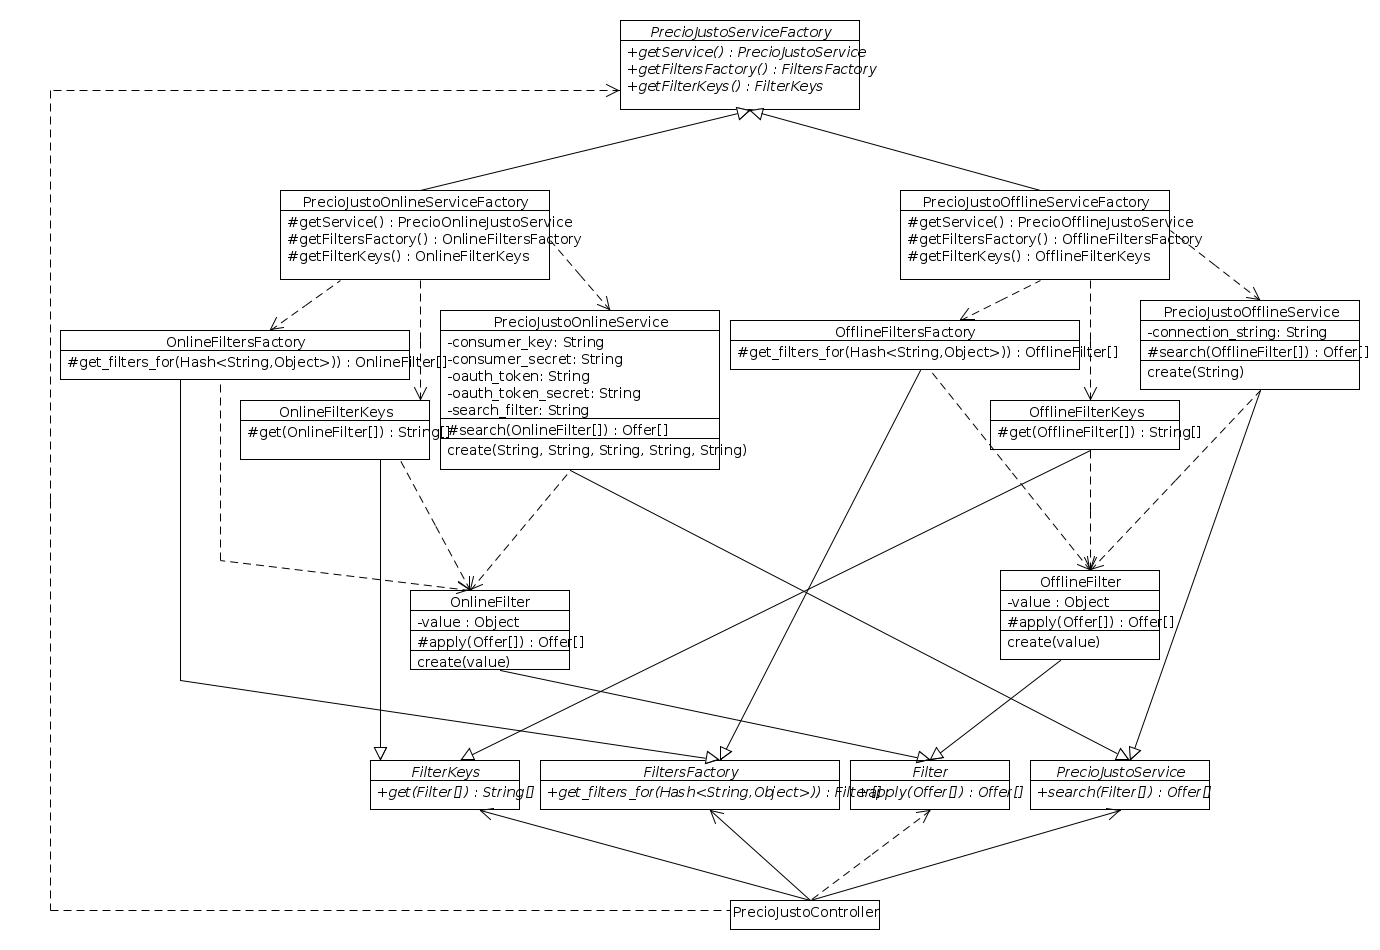
\includegraphics[width=0.8\paperwidth]{./imgs/class_diagram_service_factory_v2.png}
\caption{Diagrama de clases de creación de servicios}
\end{figure}

Dado que el filtrado de los tweets de las ofertas búscadas se realizan de distinta manera, los filtros si bien deberán proveer las misma funcionalidad son implementativamente distintos.

En un caso filtrarán las ofertas que se vayan obtienendo de twitter en vivo y en el otro caso se realizará un búsqueda sobre el motor de base de datos.

Esto puede verse en el siguiente diagrama. 

\begin{figure}[ht]
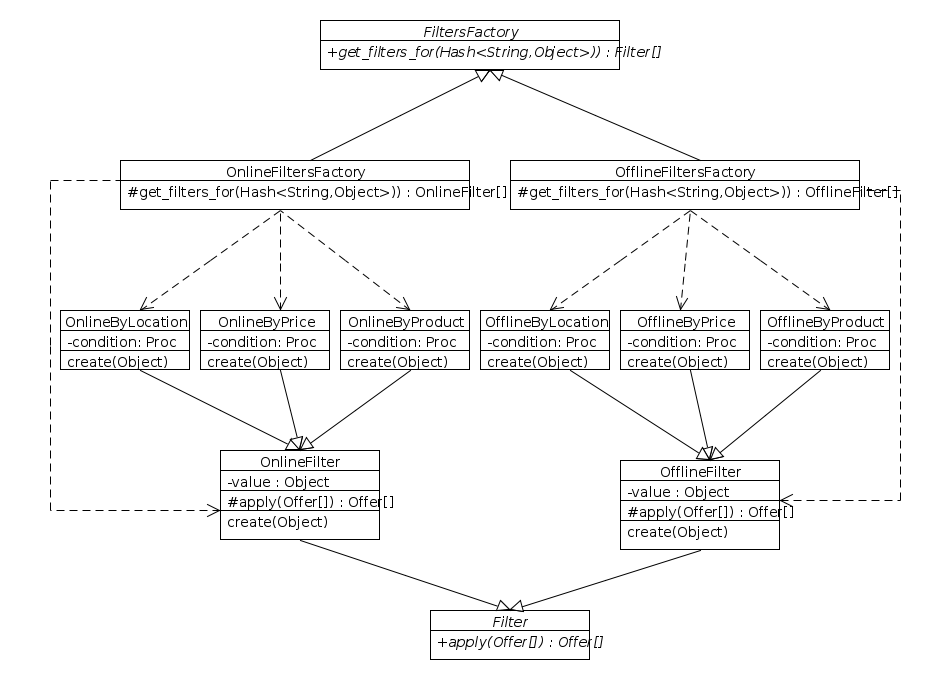
\includegraphics[width=\textwidth]{./imgs/class_diagram_filters_factory.png}
\caption{Diagrama de clases de creación de filtros}
\end{figure}

\begin{figure}[ht]
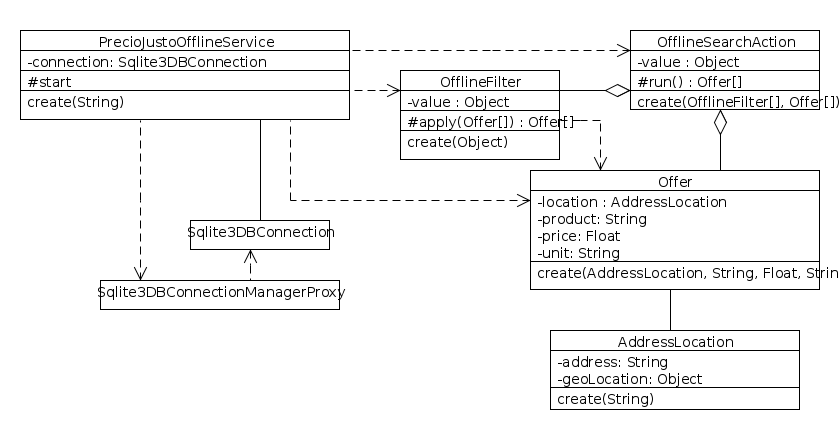
\includegraphics[width=\textwidth]{./imgs/class_diagram_offline_service.png}
\caption{Diagrama de clases de servicio offline}
\end{figure}

\begin{figure}[ht]
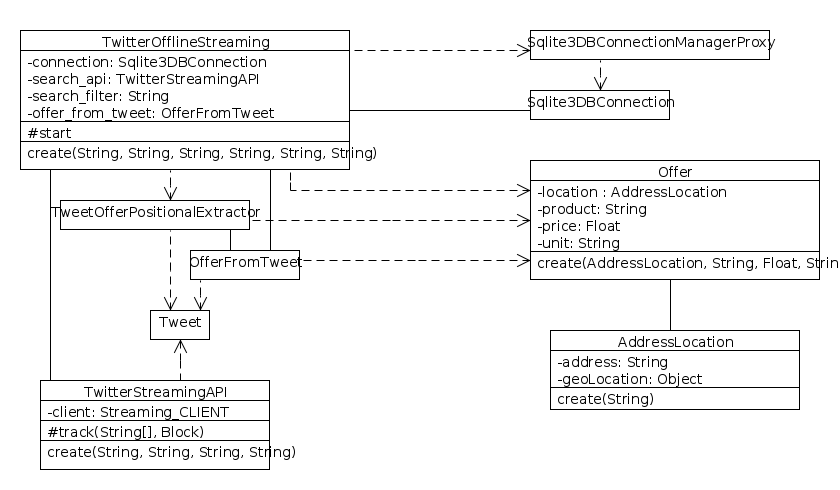
\includegraphics[width=\textwidth]{./imgs/class_diagram_offline_streaming.png}
\caption{Diagrama de clases de streaming de twitter}
\end{figure}

\begin{figure}[ht]
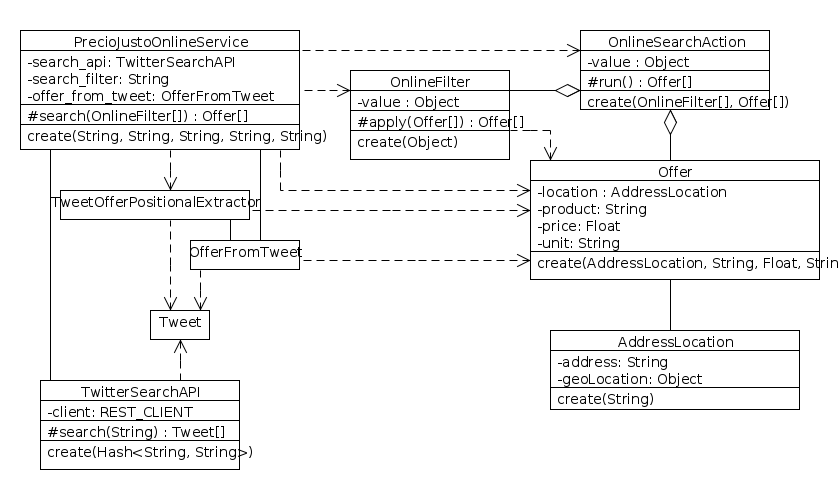
\includegraphics[width=\textwidth]{./imgs/class_diagram_online_service.png}
\caption{Diagrama de clases de servicio online}
\end{figure}

\begin{figure}[ht]
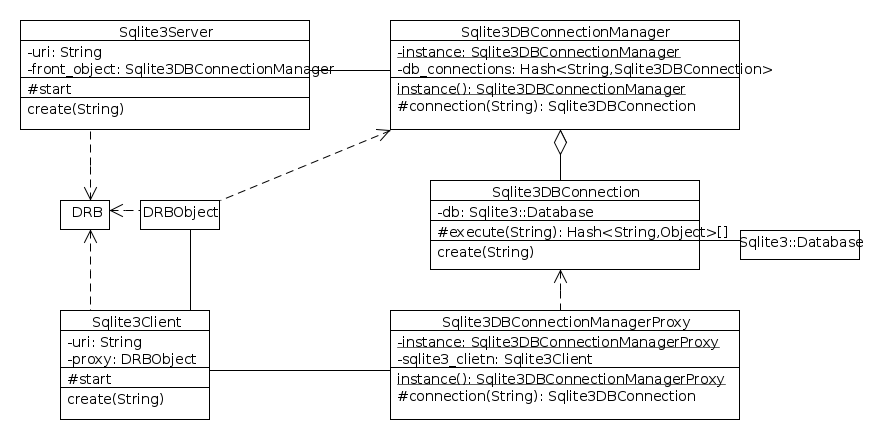
\includegraphics[width=\textwidth]{./imgs/class_diagram_sqlite3_client_server.png}
\caption{Diagrama de clases de BD SQLite3}
\end{figure}

\begin{figure}[ht]
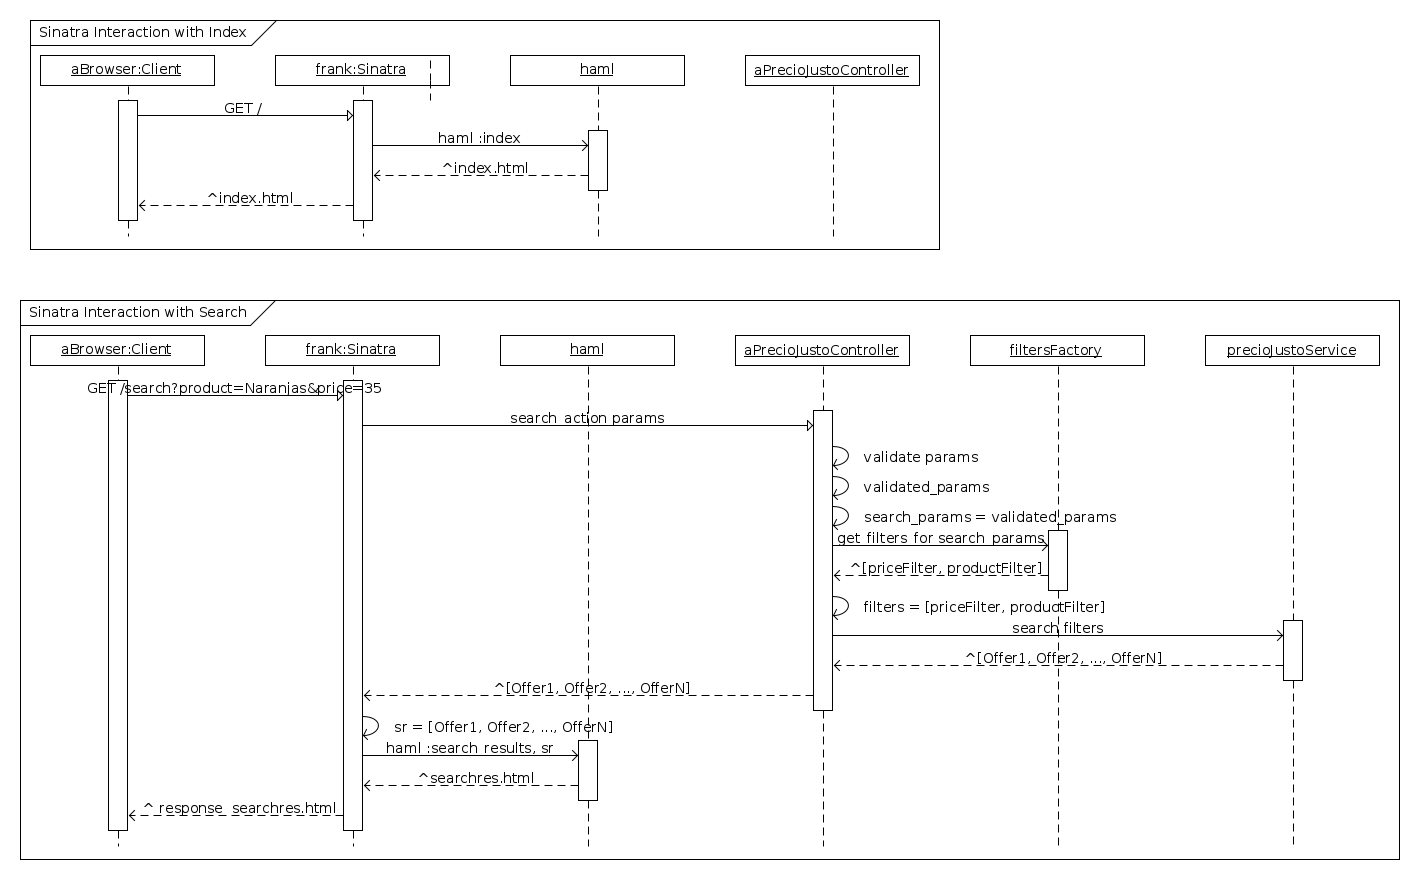
\includegraphics[width=0.8\paperwidth]{./imgs/sequence_diagram_sinatra.png}
\caption{Diagrama de secuencia de sinatra}
\end{figure}

\begin{figure}[ht]
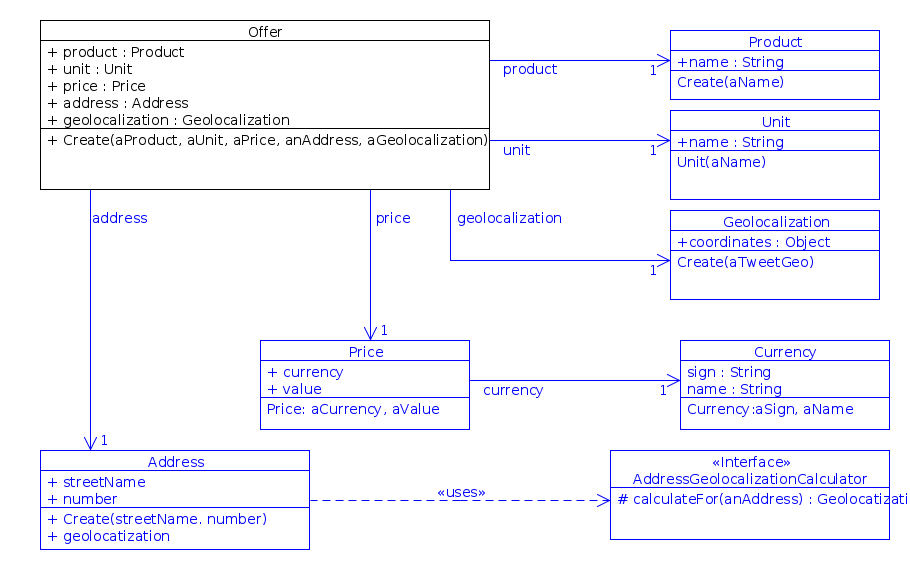
\includegraphics[width=\textwidth]{./imgs/class_diagram_offer.png}
\caption{Diagrama de clases de offer y colaboradores}
\end{figure}

\begin{figure}[ht]
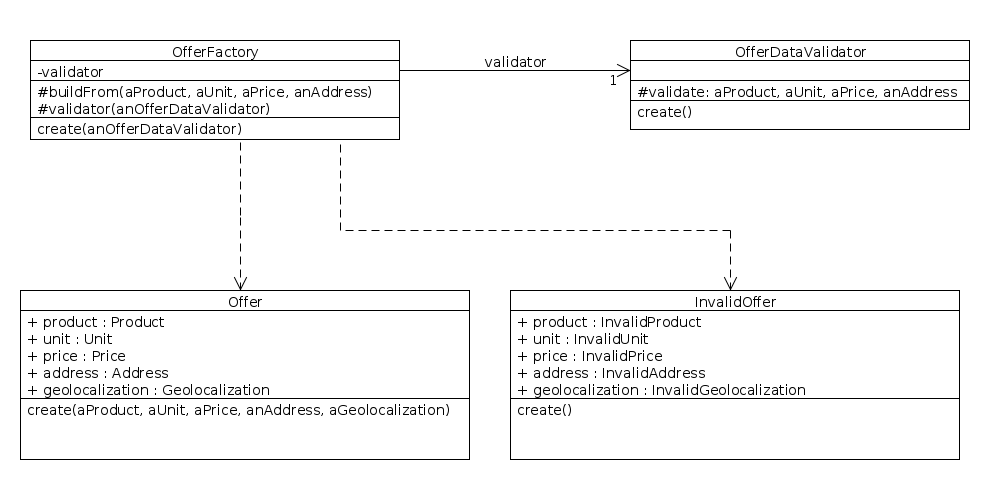
\includegraphics[width=\textwidth]{./imgs/class_diagram_Offer_Factory.png}
\caption{Diagra de clases de creación de offer}
\end{figure}

\begin{figure}[ht]
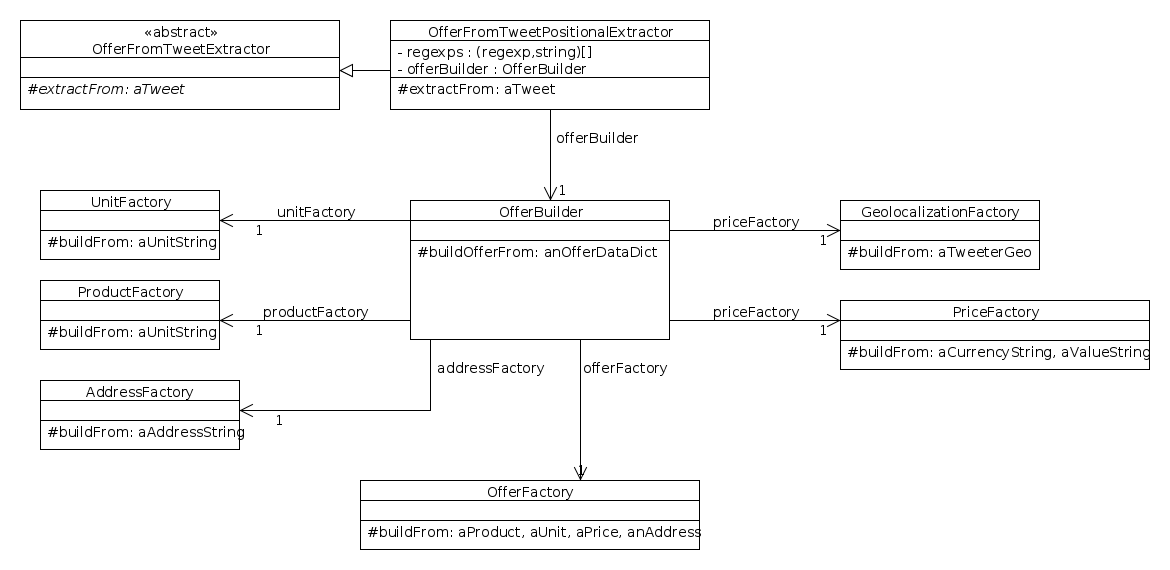
\includegraphics[width=\textwidth]{./imgs/class_diagram_parsing.png}
\caption{Diagrama de clases de extraccion datos de tweet}
\end{figure}

\begin{figure}[ht]
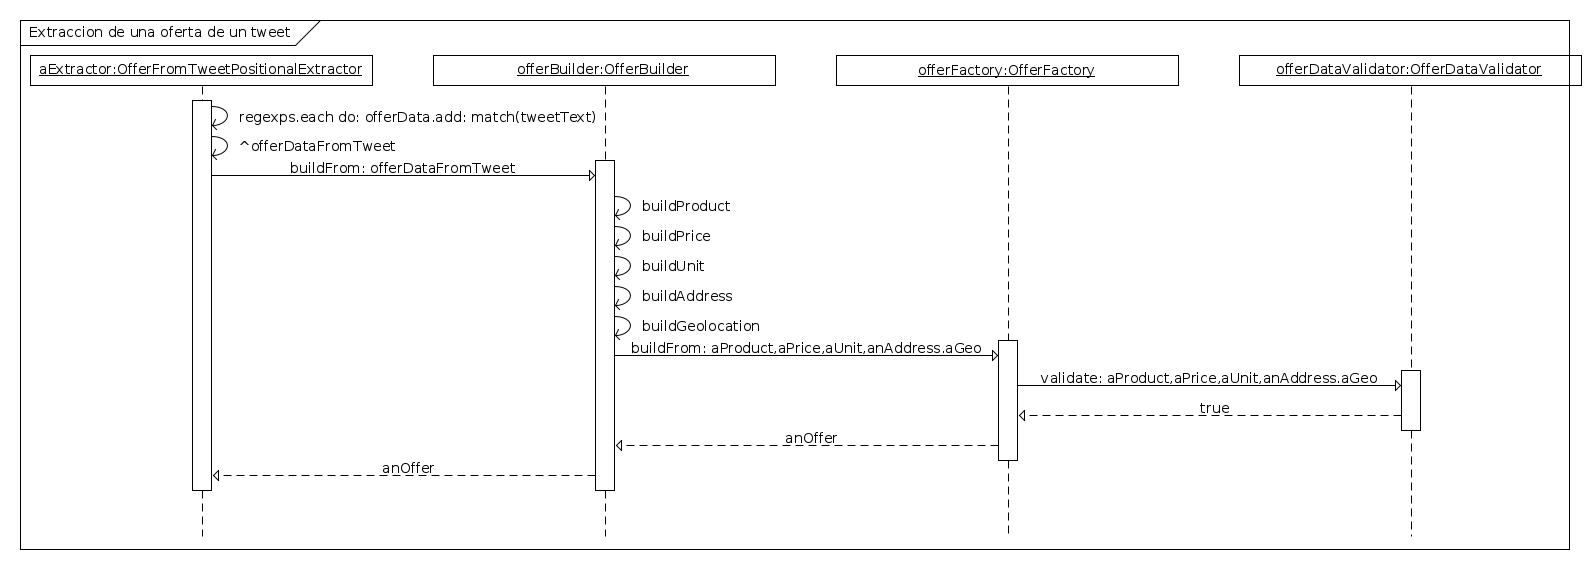
\includegraphics[width=\textwidth]{./imgs/sequence_diagram_parsing.png}
\caption{Diagrama de secuencia de extraccion de datos de tweet}
\end{figure}

